
%\subsection{The Architectural Journey: Oscillations Between Simplicity and Complexity}
%\label{subsec:TimelineArchitectureStyles}

%===========================
%%Human-Centric Design Philosophy: Explore the historical evolution of architectural philosophies that prioritize human experience and well-being. Discuss how different architectural styles and movements have addressed the balance between ornamentation, functionality, and human comfort.
%===========================
%!Concise version

Architecture stands as a unique art form, setting itself apart from other creative mediums.
It requires not only the transformation of the ordinary into the extraordinary, akin to painting and sculpture, but also the imperative to fulfill the purpose and functionality of a building~\cite{Hnin2022}.
Its evolution is marked by a dynamic interplay between simplicity and complexity, reflecting societal values and technological advancements~\cite{Economakis2023}.
As we trace the path from early architectural styles like Romanesque characterized by their robust forms and simplistic forms~\cite{Arora2023}, through to the Gothic period with their emphasis on intricate, skyward designs~\cite{Stacbond2020}, we witness the historical oscillations between simplicity and complexity that reflect changing societal values and technological advancements(see Figure~\ref{fig:Oldtimeline} a,b).

The Renaissance heralded a revival of Greek and Roman ideals and the return to symmetry, that is succeeded by the Baroque's lavish ornamentation in the 16th century~\cite{Economakis2023} (see Figure~\ref{fig:Oldtimeline} c,d).
The Neoclassical style, with its emphasis on symmetry and classical principles, dominated the 18th and 19th centuries, integrating new technologies like reinforced concrete~\cite{Economakis2023}(see Figure~\ref{fig:Oldtimeline} e).
However, its rigid academicism eventually led to more ostentatious designs, setting the stage for the emergence of Art Nouveau and Art Deco (see Figure~\ref{fig:Middletimeline} a, b).
These styles, celebrating nature and technological advancements, marked a departure from Neoclassical restraint~\cite{Salas2018, Arora2023}.

The history of Architecture reaches a pivotal moment in The 20th century with the rise of Modern Architecture, advocating `form follows function' and minimal ornamentation, marking a significant departure from the ornate designs of previous eras~\cite{Gage2015} (see Figure~\ref{fig:Middletimeline} c).
Figures such as Adolf Loos and Le Corbusier championed minimalism and functionality, influencing a generation of architects to prioritize structural honesty and simplicity~\cite{Saglam2014}.
This movement, while producing notable works, often led to uniform urban landscapes that lacked the cultural richness and diversity of their predecessors(see Figure~\ref{fig:Middletimeline} c).

In response to Modernism's perceived limitations, the late 1960s saw the emergence of Postmodernism.
Spearheaded by thinkers like Robert Venturi, Postmodernism critiqued the minimalist aesthetic and reintroduced complexity, ornament, and form into architectural design.
This movement sought to reclaim the expressiveness and symbolic richness that had been set aside by Modernist purity, advocating for buildings that engage more deeply with their cultural and historical contexts~\cite{Venturi1972} (see Figure~\ref{fig:Middletimeline} d).

The late 20th and early 21st centuries have seen a resurgence in creativity and expression, with architects utilizing digital technologies to explore new realms of complexity and ornamentation, heralding a new era of architectural design that embraces both innovation and tradition~\cite{Burlando2019} (see Figure~\ref{fig:contemporarytimeline}).

As we venture into the 21st century, the fusion of digital and physical design processes signals a shift towards the democratization of complex, parametric designs, indicative of a contemporary period that values ornamentation, functionality, and human comfort~\cite{Schwab2016}.
This evolving trajectory of architecture suggests a future where design is deeply intertwined with societal values and technological possibilities, highlighting the enduring importance of human-centric design philosophy across the ages.

%!Previous human centric design philosophy

%Architecture stands as a unique art form, setting itself apart from other creative mediums.
%It requires not only the transformation of the ordinary into the extraordinary, akin to painting and sculpture, but also the imperative to fulfill the purpose and functionality of a building\cite{Hnin2022}.
%
%At the core of architectural evolution resides a dynamic interplay between simplicity and complexity, often guided by the intersection of societal values and technological advancements\cite{Economakis2023}.
%However, it's important to clarify that within the context of this research, neither simplicity nor complexity carry any inherent negative or positive connotations.
%Using the term ``simplicity`` here doesn't imply a condemnation of one style in favor of another;
%rather, it highlights that throughout the history of architecture and its various styles, there have been periods characterized by evident complexities as well as phases where designs embraced apparent simplicities that hid their intricacies into themselves.
%Undoubtedly, every prevailing architectural style of its time has contributed masterpieces to the built environment.
%
%Consider, for instance, the transition from the robust Romanesque classic style of the 10th century, notably exhibited in churches, to the Gothic style brought by groundbreaking advancements of the 12th century that introduced buttresses, revolutionizing load distribution\cite{Arora2023}(see Figure\ref{fig:RomanesquevsGothic}).
%This innovation propelled churches skyward, inviting luminous interplays to embellish the interiors through stunning stained-glass windows bedecked in intricate design\cite{Stacbond2020}.
%
%This oscillation between complexity and simplicity persists through time— transitioning from the intricate Gothic style to the revival of Greek and Roman ideals, exemplified by the symmetrical perfection of the Renaissance era in the 14th century.
%
%This resurgence was succeeded by the opulent ornamentation and exuberance of the Baroque style in the 16th century, essentially a creation of the Chatolic church, that started in Europe and later spread across the New world in other Chatolic nations.
%It was characterized by the preference for curves over the straight line, an interest in complex plans and volumes, overlapping architectural forms, and an interest for combining the three arts of painting, sculpture and architecture\cite{Economakis2023}.
%
%The progression continued with the classical revival of the 18th century, heavily influenced by the architectural principles of classical Greece and the Palladian style.
%This revival aimed to create picturesque compositions and sought to reestablish the rational simplicity that defined ancient Greece and Rome\cite{Economakis2023}.
%
%The late 18th century marked the beginning of globalization and an information explosion, which enabled scientific advancements but also blurred the geographical origins of architectural forms.
%As a result, architectural expressions from diverse cultures became acceptable options in various contexts.
%This phenomenon led to the incorporation of multiple historical references into buildings, soon Gothic, Oriental or even Egyptian styles, to name a few, were integrated into victorian houses, resulting in stylistic confusion known as Relativism and Subjectivism.
%Architects grappled with a multitude of options and no clear consensus on architectural expression\cite{Economakis2023}.
%
%In response to this architectural chaos, the Neoclassical style would appear, envisioned under the conservative academicism of the 19th century that aimed to bring order by consolidating the architectural profession under the teachings of classical architecture as idealized during the Renaissance.
%Characterized by being bilaterally symmetrical and sel-referential or a-contextual with little regard to how they integrated to urban settings.
%This heavily inspired greek and Palladian architecture would integrate with new technologies like reinforced concrete and cast iron.
%Led by the École des Beaux-Arts in Paris, the Neoclassic style gained prominence and persisted until the early 20th century\cite{Economakis2023}.
%
%However, by the late 19th century, the increasingly rigid academicism of the École des Beaux-Arts gave way to a shift towards ostentation.
%The lack of volumetric hierarchy in building designs led to a departure from the sobriety and principles of the Renaissance.
%Their monumentality originally praised was now resulting in a tendency towards overelaboration as buildings competed for attention\cite{Economakis2023}.
%
%In the late 19th century, amidst the prevalent Neoclassical style, two influential design movements emerged: Art Nouveau and Art Deco.
%
%The Art Nouveau movement, which thrived from 1890 to 1910, celebrated nature and found its essence in organic forms.
%It was characterized by intricate and fluid designs, embracing curvilinear motifs and intricate ornamentation.
%
%Antonio Carlos Gaudí, a figure of unparalleled renown within this movement, not only exemplified the Art Nouveau style but also exhibited distinctive elements that set his work apart and positioned him ahead of his time.
%Gaudí's architectural genius extended beyond aesthetics, pioneering concepts such as sustainability and biomimetic architecture, long before these ideas took hold in architectural discourse\cite{Salas2018}(Figure\ref{fig:ArtNouveauVsModernism}).
%
%The subsequent Art Deco movement, flourishing during the 1920s and 30s, celebrated technological advancement through luxurious materials and intricate patterns.
%It blended modern design with artistic craftsmanship, embracing geometric shapes, bold colors, and streamlined forms.
%Art Deco architecture often featured sleek lines, zigzags, and stylized motifs, capturing the spirit of the era's dynamism and opulence\cite{Arora2023}.
%
%These innovative styles of the late 19th century, while revolutionary in their own right, seemed to herald an impending era of transformation.
%While not as universally embraced as the Neo-Classical style, which held sway in the 19th century, these styles indicated a shift in the broader attitude towards the teachings of the Ecole des Beaux Arts and its penchant for exuberance and monumentality.
%
%Nonetheless, the friction against the teachings of the Ecole des Beaux Arts and its reverence for exuberance reached its zenith as the 20th century unfolded.
%
%Especially prominent among architects with a more socially-minded inclination, this antagonism would pave the way for the emergence of Modern Architecture and rationalism during the first half of the 20th century.
%
%These movements brought about radical shifts in architectural paradigms, shaking the very foundations of conventional design (see Figure\ref{fig:NeoclassicalvsModernism}).
%
%%%Figure neoclassicim vs modernism
%     \begin{figure}[htb]
%          \centering
%          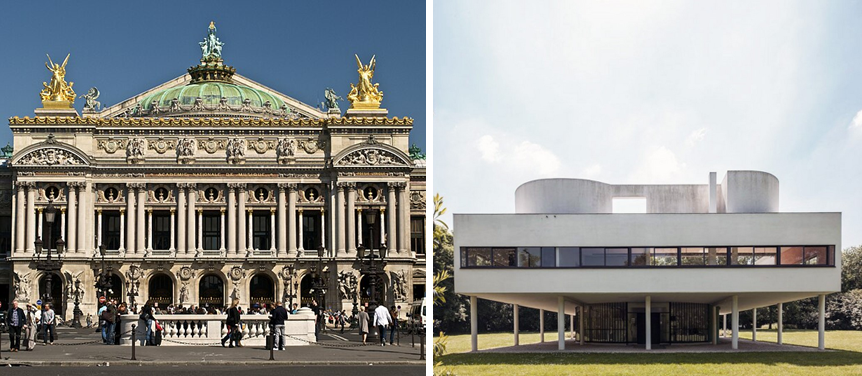
\includegraphics[width= \linewidth]{Images/NeoclassicismVsModernism}
%          \caption{Neoclassic building "Paris Opera" 19th AC (left) vs Modernist house "Villa Savoye" 20th AC (right). From Complexity to simplicity. (\textit{Images edited from source:\cite{Stacbond2020}})}
%          \label{fig:NeoclassicalvsModernism}
%        \end{figure}
%
%This architectural ethos adopted the maxim ``Form follows function'', emphasizing functionalism and characterized by a rejection of traditional ornament in favor of new forms of more subtles intricacies like the “aesthetics of machinery” that showcased architecture  enriched  with  only  the  beauty of its lines and the use of new-age materials such as steel, glass, and concrete\cite{Gage2015}.
%
%Venturi et al.\cite{Venturi1972} delve deeper into the reflections on modern architecture, which was often regarded as progressive, if not revolutionary, as well as utopian and puristic.
%They elucidate how architects of this movement, when confronted with dissatisfaction towards existing conditions, often leaned towards tearing down and rebuilding, rather than seeking to enhance or adapt what already existed.
%
%This tendency for radical transformation rather than gradual evolution underscores the assertive and sometimes uncompromising nature of modernist architectural interventions.
%
%%% add some extra references to the modernist section specially about the urban configuration
%
%The postmodernism style of the late 60's marks a radical return of ornament in form recognizing that even simplified modern elements serve as ornamentation focusing on the thought of freeing design element from oppresive modern constraints.
%
%
%
%The late 20th century embraced imagination and expression through architects like Frank Gehry, Zaha Hadid, and Rem Koolhaas.
%Their constructions stood as monumental expressions of ornament, enabled by digital technologies (Figure\ref{fig:Modernismvspostmodernism}).
%%
%%%Figure neoclassicim vs modernism
%     \begin{figure}[htb]
%          \centering
%          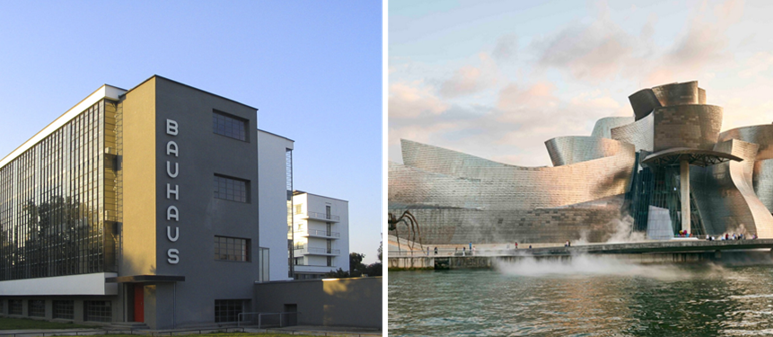
\includegraphics[width= \linewidth]{Images/modernism vs postmodernism}
%          \caption{Modernist building "Bauhaus School" 20th AC (left) vs Postmodernist "Guggenheim museum" 1997 (right). From simplicity to Complexity. (\textit{Images edited from source:\cite{Arora2023}})}
%          \label{fig:Modernismvspostmodernism}
%        \end{figure}
%
%Intricate shapes and structures have materialized, spanning from juxtaposed ornaments to innovative transformative structural ornamentation.
%This pursuit of complexity is a global phenomenon, prompting a competitive quest among leading contemporary architectural firms to harness parametric design as a tool to conceive groundbreaking new buildings.\cite{Burlando2019}.
%
%However, due to their complexity, these structures remained exceptional, not integrated into the urban fabric.
%Now at the beginning of the 21st century and the advent of the 4th industrial revolution, characterized by a fusion of technologies that is blurring the lines between the physical, digital, and biological spheres\cite{Schwab2016}, forecasts the democratization of digital fabrication which in turn will bring a paradigm shift, offering globally to all cultures the means to express authenticity through complex parametric designs, signaling a contemporary era embracing complexity and ornament.
%
%Amidst this historical exploration, it becomes evident that the architecture of the future is poised to harmonize ornamentation, functionality, and human comfort.
%The trajectory points towards a style of complexity—a style that crafts a delicate equilibrium, resonating with the values of our time and the technological possibilities at our fingertips.
%
%In this intricate interplay, architecture emerges as a tangible synthesis of human experience and creative expression, balancing ornament's aesthetic allure, the essential functionality of the built environment, and the crucial comfort of its inhabitants.
